\documentclass{article}
\usepackage{amsmath}
\usepackage{amsfonts}
\usepackage{amssymb}
\usepackage{tcolorbox}
\usepackage[inline]{enumitem}
\usepackage[a4paper,margin=1in]{geometry}
\usepackage[normalem]{ulem}
\usepackage{graphicx}
\usepackage{tasks}
\settasks{label=(\alph*), label-offset=0.4em, label-width=1.5em}

\usepackage{fancyhdr}
\fancyhf{}
\setlength{\headheight}{36pt}
\renewcommand{\headrulewidth}{0pt}
\thispagestyle{fancy}
\lhead{Calculus Exercise}
\chead{Week 12 (7.1, 7.2, 7.3)}
\rhead{\underline{ID:\hspace{7.4em}} \\ \vspace{0.2cm} \uline{Name:\hspace{6em}}}
\cfoot{\thepage}

\begin{document}
\begin{enumerate}
\item[7.1.2]
    Evaluate the integral using integration by parts with the indicated choices of $u$
    and $dv$.
    \[
        \int \sqrt{x} \ln x dx;\ u = \ln x,\ dv = \sqrt{x}dx
    \]

\vspace{5cm}

\item[7.1.48]
    First make a substitution and then use integration by parts to evaluate the integral.
    \[
        \int_{}^{} \frac{\sin^{-1} (\ln x)}{x} dx
    \]

\vspace{5cm}

\item[7.1.54]
    Prove the reduction formula.
    \begin{enumerate}
        \item
        \[
            \int \cos^{n} x dx = \frac{1}{n} \cos^{n-1} x \sin x
            + \frac{n-1}{n}\int \cos^{n-2} x dx
        \]
        \item Use part (a) to evaluate $\displaystyle \int \cos^{2} x dx$.
        \item Use parts (a) and (b) to evaluate $\displaystyle \int \cos^{4} x dx$.
    \end{enumerate}

\newpage

\item[7.1.60]
    Use integration by parts to prove the reduction formula.
    \[
        \int \sec^{n} x dx = \frac{\tan x \sec^{n-2} x }{n-1}
        + \frac{n-2}{n-1}\int \sec^{n-2} x dx\ ( n \neq 1 )
    \]

\vspace{5cm}

\item[7.1.78]
    \begin{enumerate}
        \item Use integration by parts to show that
        \[
            \int f(x) dx = x f(x) - \int xf'(x) dx
        \]
        \item If $f$ and $g$ are inverse functions and $f'$ is
            continuous, prove that
        \[
            \int_{a}^{b} f(x) dx = b f(b) - a f(a) -
            \int_{f(a)}^{f(b)} g(y) dy
        \]
        \item In the case where $f$ and $g$ are positive functions and
            $b > a > 0$, draw a diagram to give a geometric
            interpretation of part (b).
        \item Use part (b) to evaluate $\displaystyle \int_{1}^{e} \ln x dx$.
    \end{enumerate}

\vspace{6cm}

\item[7.2.32]
    Evaluate the integral.
    \[
        \int \tan^{2}x \sec x dx
    \]
\newpage

\item[7.2.56]
    Evaluate the integral.
    \[
        \int \frac{1}{1 + \sec \theta} d\theta
    \]

\vspace{8cm}

\item[7.2.62]
    \begin{enumerate}
        \item Prove the reduction formula
        \[
            \int \tan^{2n} x dx = \frac{\tan^{2n-1} x }{2n-1}
            - \int \tan^{2n-2} x dx
        \]
        \item Use this formula to find $\displaystyle  \int \tan^{8}x dx$
    \end{enumerate}

\newpage

\item[7.2.63]
    Find the average value of the function $f(x) = \sin^{2}x \cos^{3}x$
    on the interval $[-\pi , \pi]$.

\vspace{6cm}

\item[7.2.71]
    Find the volume obtained by rotating the region bounded by the
    curves about the given axis.
    \[
        y = \sin x,\ y = \cos x,\
        0 \leqslant x \leqslant \frac{\pi}{4};\ \text{ about } y= 1
    \]

\vspace{6cm}

\item[7.3.30]
    Evaluate the integral.
    \[
        \int_{0}^{1} \sqrt{x-x^{2}} dx
    \]

\newpage

\item[7.3.44]
    Find the volume of the solid obtained by rotating about the
    the line $x=1$ the region under the curve
    $y = x \sqrt{1-x^{2}},\ 0 \leqslant x \leqslant 1$.

\vspace{7cm}

\item[7.3.45]
    \begin{enumerate}
        \item Use trigonometric substitution to verify that
        \[
            \int_{0}^{x} \sqrt{a^{2}-t^{2}}dt
            = \frac{1}{2} a^{2} \sin^{-1} \left(\frac{x}{a}\right)
            + \frac{1}{2}x \sqrt{a^{2}-x^{2}}
        \]
        \item Use the figure to give trigonometric interpretations of
            both terms on the right side of the equation in part (a).
    \end{enumerate}

    \begin{center}
        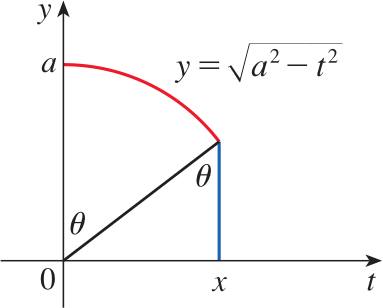
\includegraphics[height=4cm]{./png/7.3.45.png}
    \end{center}

\newpage

\item[7.3.47]
    A torus is generated by rotating the circle $x^{2}+(y-R)^{2}= r^{2}$
    about the $x$-axis. Find the volume enclosed by the torus.

\end{enumerate}
\end{document}
